
%%% Local Variables:
%%% mode: latex
%%% TeX-master: t
%%% End:

\chapter{Spark 弹性分布式数据集与 MLlib}
\label{cha:spark_RDD_mllib}
Spark 是一个基于 MapReduce 的通用的大数据并行计算框架,最初由 UC Berkeley AMP Lab 开发。Spark 的架构是在 Hadoop 基础上的改良,继承了 MapReduce 的优点,它与 Hadoop 最大不同之处就是内存计算,Hadoop 将计算过程的中间数据存储在磁盘上,而 Spark 一般是用内存来存储数据,所有数据操作都在内存中完成。
\begin{figure}[H]
  \centering
  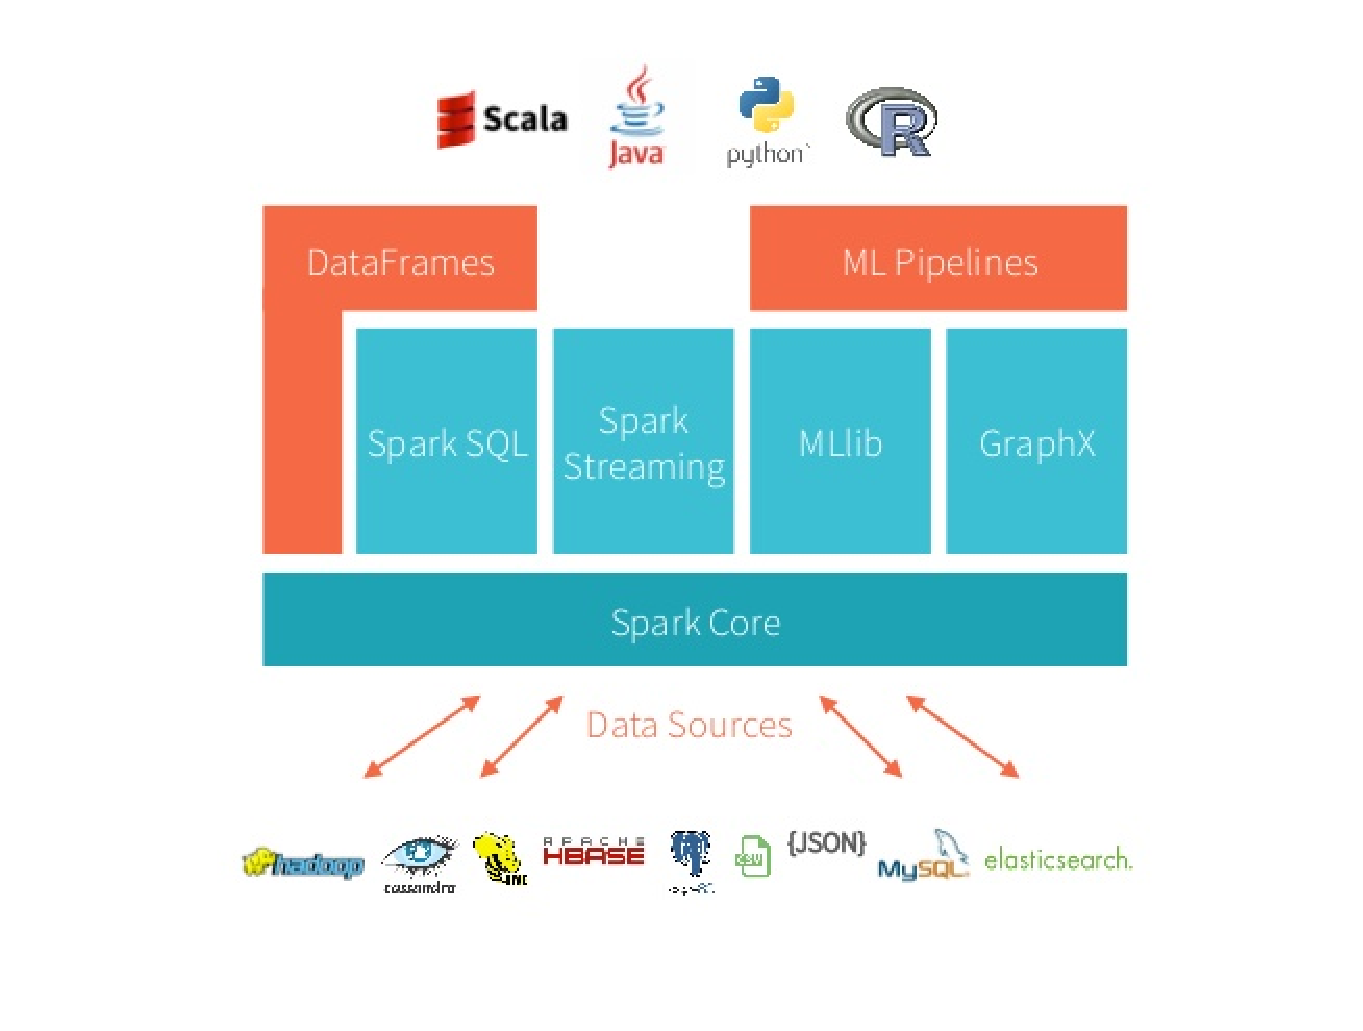
\includegraphics[width=1.0\linewidth]{spark-core}
  \caption{Spark 生态圈}
  \footnotesize 注:图像来源\protect\footnotemark
\end{figure}
\footnotetext{http://www.slideshare.net/rxin/stanford-cs347-guest-lecture-apache-spark?utm\_source=tuicool}
在 Spark 的生态圈中,Spark 的数据来源可以不仅可以从本地系统或者 HDFS 上各种格式的数据,还可以从 HBase、Cassandra 等数据库中的数据。基于在 Spark 的内核,还提供了诸如 Spark Streaming、Spark SQL、MLlib、GraphX 等数据处理的库。开发者可以使用 Scala、Java、Python 甚至是 R 语言编写 Spark 应用程序完成数据处理的任务。
\section{弹性分布式数据集}
弹性分布式数据集(Resilient Distributed Datasets,下文简称 RDD)\cite{Zaharia2012}是 Spark 中的分布式内存的抽象。相比于 Hadoop 中的计算过程,RDD 可以被缓存在内存当中,每一次的计算产生的结果都可以保留在内存当中。对于迭代计算,这样多次迭代的计算每次可以将结果保存在内存中,下一次迭代又可以直接从内存中读取数据计算,从而避免了大量的磁盘读写操作,大大节省了计算时间。

一般来说,RDD 的创建是通过 SparkContext 来实现,主要包含有两种创建来源:一是从支持的文件系统(或支持的数据库)读取创建;二是从内存数据集合生成。不同于 Hadoop 中仅有 Map 和 Reduce 操作,RDD 还支持其他类型的操作,主要分为转换操作、控制操作和行为操作三类。转换操作顾名思义,就是将一个 RDD 操作之后转换为另一个 RDD,包括 map、flatMap、filter 等操作。控制操作主要用来将 RDD 缓存到内存中或者磁盘上,比如 cache、persist、checkpoint等操作。行为操作主要分为两类:一类是变成集合或标量的操作,另一类是将 RDD 外部文件系统或数据库的操作。Spark 中的所有对 RDD 的操作,只有当执行行为操作时,才会执行之前的转换或控制操作。例如,我们先对 RDD 执行 map 操作, 然后执行 reduce 操作, 在 map 操作时,Spark 并不会真正执行,只是记录,只有执行 reduce 操作时才会真正一起计算。这一特性称为惰性计算(lazy computing)。图(\ref{fig:rdd})展示的 RDD 的一个操作流程。
\begin{figure}[H]
  \centering
  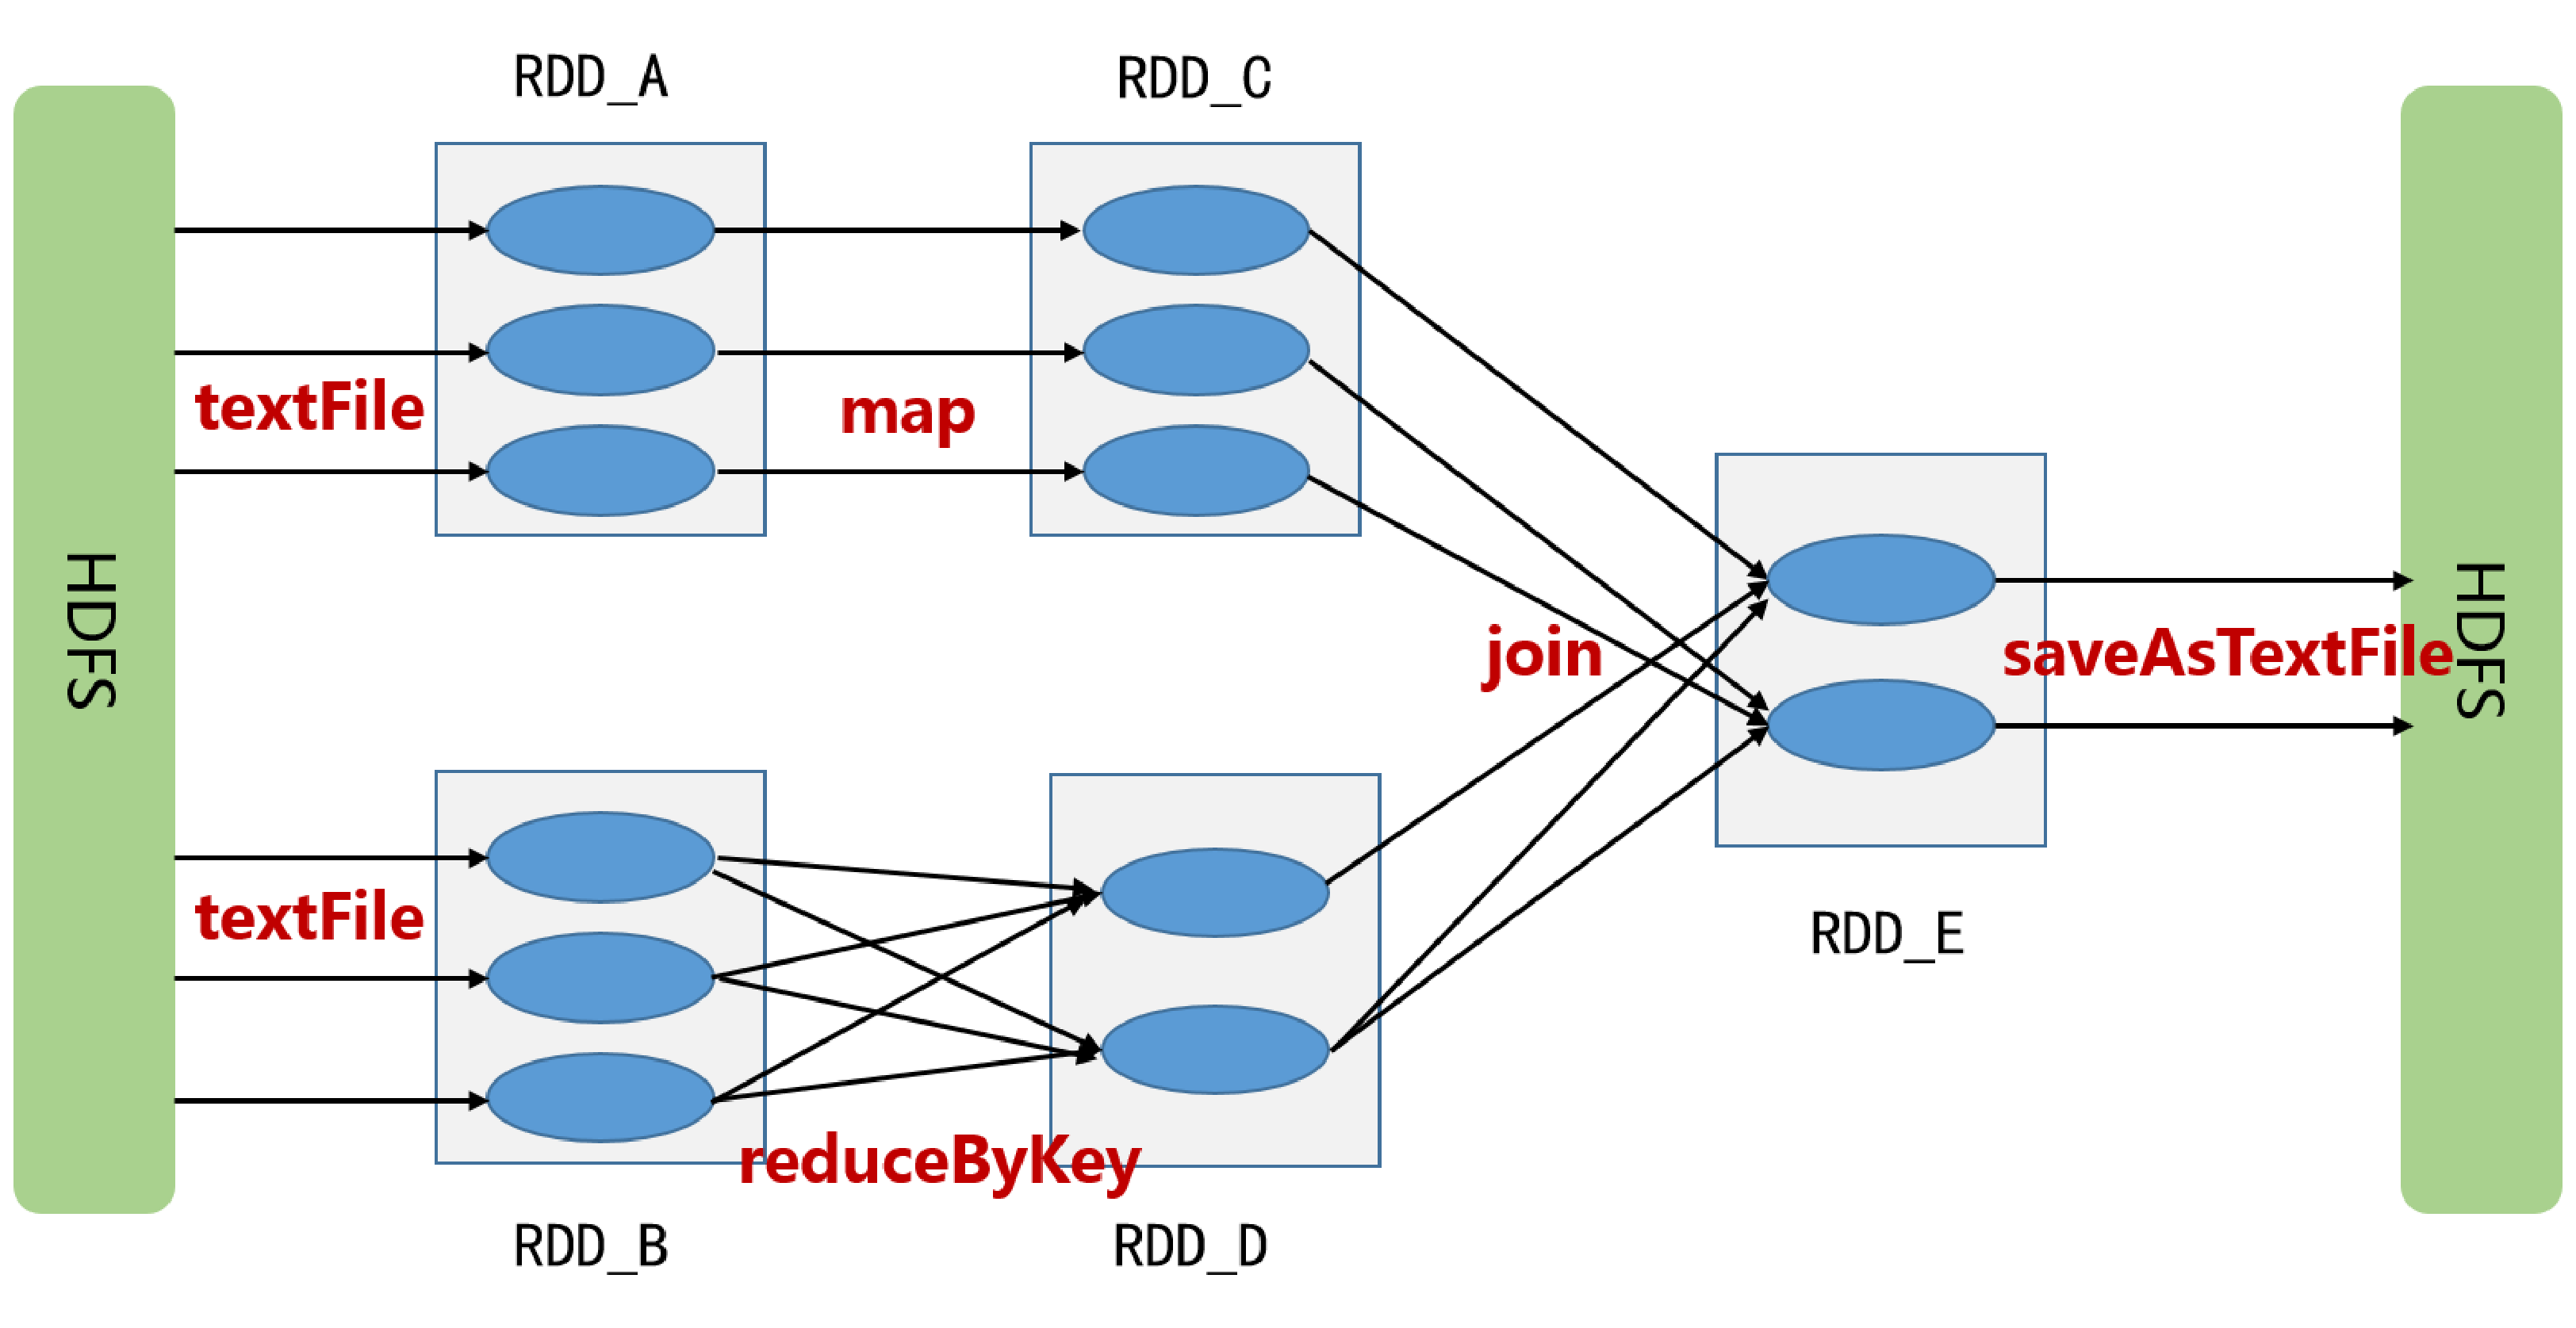
\includegraphics[width=1.0\linewidth]{rdd}
  \caption{RDD 操作流程示例}
  \label{fig:rdd}
\end{figure}

RDD 的持久化是 Spark 中 RDD 的一个重要特性。通过 RDD 的持久化,我们可以将 RDD 缓存到内存或者磁盘上。默认地,RDD 并不会进行缓存,每次计算需要用到 RDD 时,都需要重新计算获取 RDD,这样是非常低效的,特别是对于一些迭代的计算。因此,我们需要考虑在计算过程中,将一些重复用到的 RDD 进行缓存操作,这样我们我们只要第一次计算出 RDD,以后每次用到相同的 RDD 时就不用在重复计算,从缓存中直接读取就可以了。RDD 的 cache() 和 persist() 函数就是用于缓存的,其中 cache() 函数是指将 RDD 缓存在内存当中,而 persist() 根据参数可以将 RDD 进行不同级别的缓存。
RDD 本身自带有容错机制,通过记录 RDD 的演变过程以便在任务执行失败的时候能够恢复出原有的数据,而不需要通过备份的形式实现容错。例如,当前的 RDD 的因任务执行失败而数据丢失,系统则会根据记录的 RDD 演变关系回溯到未丢失的祖先 RDD,重新根据转换操作计算出一个新的 RDD 进行恢复。
\section{MLlib}
随着数据量的不断增大,传统的单机式的机器学习算法实现已经无法满足大数据的要求,分布式机器学习算法为解决大数据机器学习的提供了可能。MLlib 是基于 Spark 构建的一个常用分布式机器学习算法和工具库,目前支持的算法包括分类算法、回归算法、聚类算法、协同过滤算法、降维算法等。MLlib 中的分布式机器学习算法,相比于以往的算法,在时间效率有了明显提升。下图(\ref{fig:logistic-regression})是逻辑回归算法在 Hadoop 和 Spark 上的执行时间对比。
\begin{figure}[H]
  \centering
  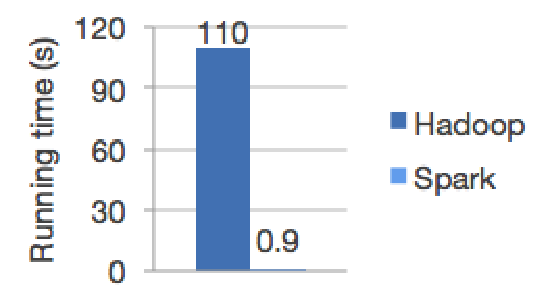
\includegraphics[width=0.3\linewidth]{logistic-regression}
  \caption{Hadoop 和 Spark 上逻辑回归算法效率对比}
  \label{fig:logistic-regression}
  \footnotesize 注:图像来源\protect\footnotemark
\end{figure}
\footnotetext{http://spark.apache.org/}
MLlib 中已经实现的一些常用机器学习算法可以供使用者调用,在 Spark 实现分布式地实现大规模数据的机器学习的任务正是一个不错的选择。

